\documentclass[11pt]{beamer}
\usepackage[utf8]{inputenc}
\usepackage{graphicx} 
\usepackage{booktabs} 

\mode<presentation> {
\usetheme{Madrid}
%\usecolortheme{albatross}
}

\title[]{Optical Flow: Lucas–Kanade Method}
\author[]{George Tang, Jerry Liu} 
\institute[]{Thomas Jefferson High School for Science and Technology} 

\begin{document}

\begin{frame}
\titlepage 
\end{frame}

\begin{frame}{Introduction}
\begin{itemize}
    \item Given a sequence of images over a short duration of time, \textbf{Optical Flow} allows us to track the \textbf{apparent motion} 
    \item Apparent motion is caused by the relative motion between an observer and the scene
    \item Applications in computational photography
\end{itemize}
\begin{figure}
    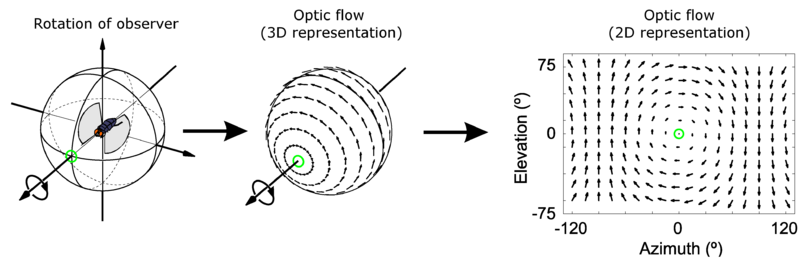
\includegraphics[width=0.8\textwidth]{optical1.png} \\
    \caption{Optical Flow from the Perspective of the Fly}
\end{figure}
\end{frame}


\begin{frame}{Brightness Constancy Constraint}
\begin{itemize}
    \item Optical flow assumes a \textbf{Brightness Constancy Constraint}
    \item The lighting is invariant between frames, so the brightness of each pixel remains the same. Mathematically, we can write
\end{itemize}
$$ I(x, y, t-1) = I(x+\Delta x, y+\Delta y, t)$$

\begin{itemize}
    \item where $\Delta x$ and $\Delta y$ are the horizontal and vertical motions of the pixel and $t$ timestamp.
    \item Motion is small $\rightarrow$ local linear approximation. Consider our brightness function
\end{itemize}
$$ I(x(t), y(t), t)$$

$$ \frac{dI(x(t), y(t), t)}{dt} = \frac{\partial I}{\partial x}\frac{dx}{dt} + \frac{\partial I}{\partial y}\frac{dy}{dt} + \frac{\partial I}{\partial t}$$
\end{frame}

\begin{frame}{Brightness Constancy Constraint (continued)}
\begin{itemize}
    \item So our approximation becomes
\end{itemize}
$$I(x+\Delta x, y+\Delta y, t) = I(x, y, t-1) + \frac{dI(x(t), y(t), t)}{dt} $$

$$I(x+\Delta x, y+\Delta y, t) = I(x, y, t-1) + \frac{\partial I}{\partial x}\frac{dx}{dt} + \frac{\partial I}{\partial y}\frac{dy}{dt} + \frac{\partial I}{\partial t}$$

\begin{itemize}
    \item And because the brightness remains the same... where  $I_x$ = $\frac{\partial I}{\partial x}$, u = $\frac{dx}{dt}$, etc. Note we are interested in $u$ and $v$.
\end{itemize}
$$ \frac{\partial I}{\partial x}\frac{dx}{dt} + \frac{\partial I}{\partial y}\frac{dy}{dt} + \frac{\partial I}{\partial t} = 0$$

$$ I_xu + I_yv + I_t  = 0$$
$$ I_xu + I_yv = -I_t$$
\end{frame}

\begin{frame}{Lucas–Kanade Method}
\begin{itemize}
    \item Assumes a local patch of pixels moves in the same way ($u$ and $v$ are the same)
    \item E.g. 3x3 patch yields 9 equations $\rightarrow$ over-constrained system
\end{itemize}

$$ I_x(x_0, y_0)u + I_y(x_0, y_0)v = -I_t(x_0, y_0)$$
$$ I_x(x_1, y_1)u + I_y(x_1, y_1)v = -I_t(x_1, y_1)$$
$$&\;\;\vdots \notag$$ \\
$$ I_x(x_n, y_n)u + I_y(x_n, y_n)v = -I_t(x_n, y_n)$$
\\
\end{frame}

\begin{frame}{Lucas–Kanade Method (continued)}
\begin{itemize}
    \item This system can be written in matrix form as $Am = b$
\end{itemize}
\begin{center}
\[ A =  \begin{bmatrix}
I_x(x_0, y_0) & I_y(x_0, y_0) \\
I_x(x_1, y_1) & I_y(x_1, y_1) \\
\;\;\vdots \notag  &  \;\;\vdots \notag \\
I_x(x_n, y_n)  & I_y(x_n, y_n)
\end{bmatrix} 
%
\hspace{10pt}
m = 
\begin{bmatrix}
u \\
v 
\end{bmatrix}
%
\hspace{10pt}
b = 
\begin{bmatrix}
-I_t(x_0, y_0) \\ 
-I_t(x_1, y_1) \\ 
\;\;\vdots \notag \\
-I_t(x_n, y_n)
\end{bmatrix}
\]
\end{center}
\end{frame}

\begin{frame}{Least Squares Approximation}
\begin{itemize}
    \item Solve using Least Squares Approximation
\end{itemize}
$$ Am = b $$
$$ A^TAm = A^Tb $$
$$ m = (A^TA)^{-1}A^Tb$$

\begin{center}
\[
\begin{bmatrix}
u \\ 
v 
\end{bmatrix}
% 
=
\\
\begin{bmatrix}
\sum_i{I_x(x_i, y_i)^2} & \sum_i{I_x(x_i, y_i)I_y(x_i, y_i)} \\ 
\sum_i{I_x(x_i, y_i)I_y(x_i, y_i) & \sum_i{I_y(x_i, y_i)^2}}
\end{bmatrix}
% 
\begin{bmatrix}
-\sum_i{I_x(x_i, y_i)I_t(x_i, y_i)} \\
-\sum_i{I_y(x_i, y_i)I_t(x_i, y_i)}
\end{bmatrix}
\]
\end{center}

\end{frame}

\begin{frame}{Example}
    \begin{figure}
    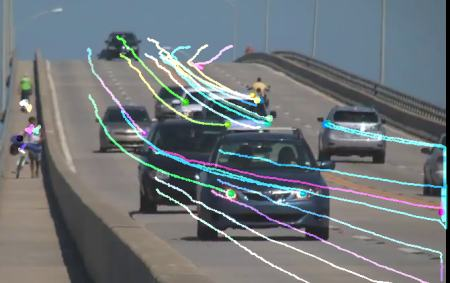
\includegraphics[width=0.8\textwidth]{opticalflow_lk.jpg} \\
    \caption{Optical Flow with Lucas-Kanade}
\end{figure}
\end{frame}

\end{document}